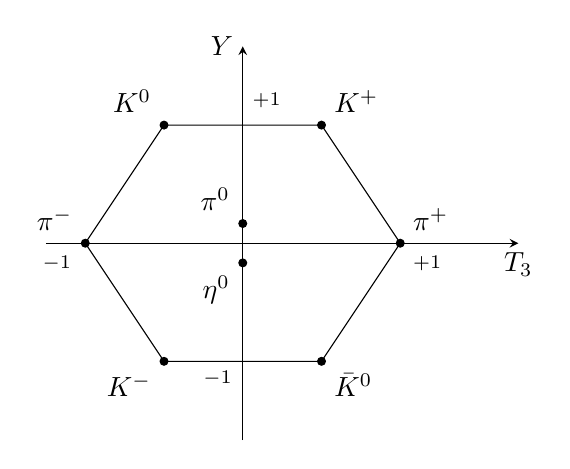
\begin{tikzpicture}[>=stealth,
  punto/.style={circle, draw=\MinorColor, fill=\MinorColor, inner sep=1pt}]
  \draw[->] (-2.5,0) -- (3.5,0) node [below] {$T_3$};
  \draw[->] (0,-2.5) -- (0,2.5) node [left] {$Y$};
  \draw (1,1.5) node [punto, label=above right:$K^+$] {}
     -- (2,0) node [punto, label=below right:$^{+1}$, label=above right:$\pi^+$] {}
	 -- (1,-1.5) node [punto, label=below right:$\bar{K}^0$] {}
     -- (-1,-1.5) node [punto, label=below left:$K^-$] {}
     -- (-2,0) node [punto, label=below left:$^{-1}$, label=above left:$\pi^-$] {}
     -- (-1,1.5) node [punto, label=above left:$K^0$] {} -- cycle;
  \node (a) at (0,1.5) [above right] {$^{+1}$};
  \node (b) at (0,-1.5) [below left] {$^{-1}$};
  \node (p) at (0,.25) [punto, label=above left:$\pi^0$] {};
  \node (e) at (0,-.25) [punto, label=below left:$\eta^0$] {};
\end{tikzpicture}
